\documentclass[11pt]{article}
 
\usepackage[margin=.95in]{geometry} 
\usepackage{amsmath,amsthm,amssymb, graphicx, multicol, array}
 
\newcommand{\N}{\mathbb{N}}
\newcommand{\Z}{\mathbb{Z}}
 

\begin{document}
 
\title{Homework 1}
\author{Juliette Franqueville\\
}
\maketitle

\subsection*{(1)  For $y_1,.., y_n \sim \mathcal{N}(\mu,\sigma^2 )$, show that $s = (\bar{y},s^2 )$ are sufficient. Also, find the observed and the expected information matrices}

The factorization theorem says that statistic $s$ is sufficient iif $f(y_{1:n}|\theta) = g(s|\theta)h(y_{1:n})$. For the normal, we have:

\begin{align*}
   f(y_{1:n}|\theta) &= \prod (2\pi \sigma^2)^{-1/2} \text{exp}\left(-\frac{(y_i-\mu)^2}{2\sigma^2}\right) \\
   &=(2\pi \sigma^2)^{-n/2}\text{exp}\left(-\frac{\sum (y_i-\mu)^2}{2\sigma^2}\right) \\
    &=(2\pi \sigma^2)^{-n/2}\text{exp}\left(-\frac{\sum ([y_i-\bar{y}]-[\mu-\bar{y})]^2}{2\sigma^2}\right) \\
    &=(2\pi \sigma^2)^{-n/2}\text{exp}\left(-\frac{\sum \{ [y_i-\bar{y}]^2-2[y_i-\bar{y}][\mu-\bar{y}]+[\mu-\bar{y}]^2 \}}{2\sigma^2}\right) \\
        &=(2\pi \sigma^2)^{-n/2}\text{exp}\left(-\frac{\sum \{ [y_i-\bar{y}]^2+[\mu-\bar{y}]^2 \}}{2\sigma^2}\right) \\
        &=(2\pi \sigma^2)^{-n/2}\text{exp}\left(-\frac{\sum  [y_i-\bar{y}]^2}{2\sigma^2}\right) \text{exp}\left(-\frac{n [\mu-\bar{y}]^2}{2\sigma^2}\right) \\
        &=(2\pi \sigma^2)^{-n/2}\text{exp}\left(-\frac{\sum  [y_i-\bar{y}]^2}{2\sigma^2}\right) \text{exp}\left(-\frac{n [\mu-\bar{y}]^2}{2\sigma^2}\right) \\
    &=(2\pi \sigma^2)^{-n/2}\text{exp}\left(-\frac{(n-1)s^2}{2\sigma^2}\right) \text{exp}\left(-\frac{n [\mu-\bar{y}]^2}{2\sigma^2}\right) \\
\end{align*}


We recognize $h(y_{1:n}) =1 $ and $g(\bar{y}, s^2|\mu, \sigma^2)= (2\pi \sigma^2)^{-n/2}\text{exp}\left(-\frac{(n-1)s^2}{2\sigma^2}\right) \text{exp}\left(-\frac{n [\mu-\bar{y}]^2}{2\sigma^2}\right)$ is a sufficient statistic for $(\mu, \sigma^2)$.


\subsection*{(3)  (a) Draw a random sample of size $n = 2$0 from a $\text{Cauchy}(0,1)$ distribution. Compute $\bar{y}n$. Repeat this $B = 1000$ times. Draw a histogram of the sampled $\bar{y}n$ values, superimposed over a $\text{Cauchy(0,1)}$ density.}

\begin{figure}[!h]
    \centering
    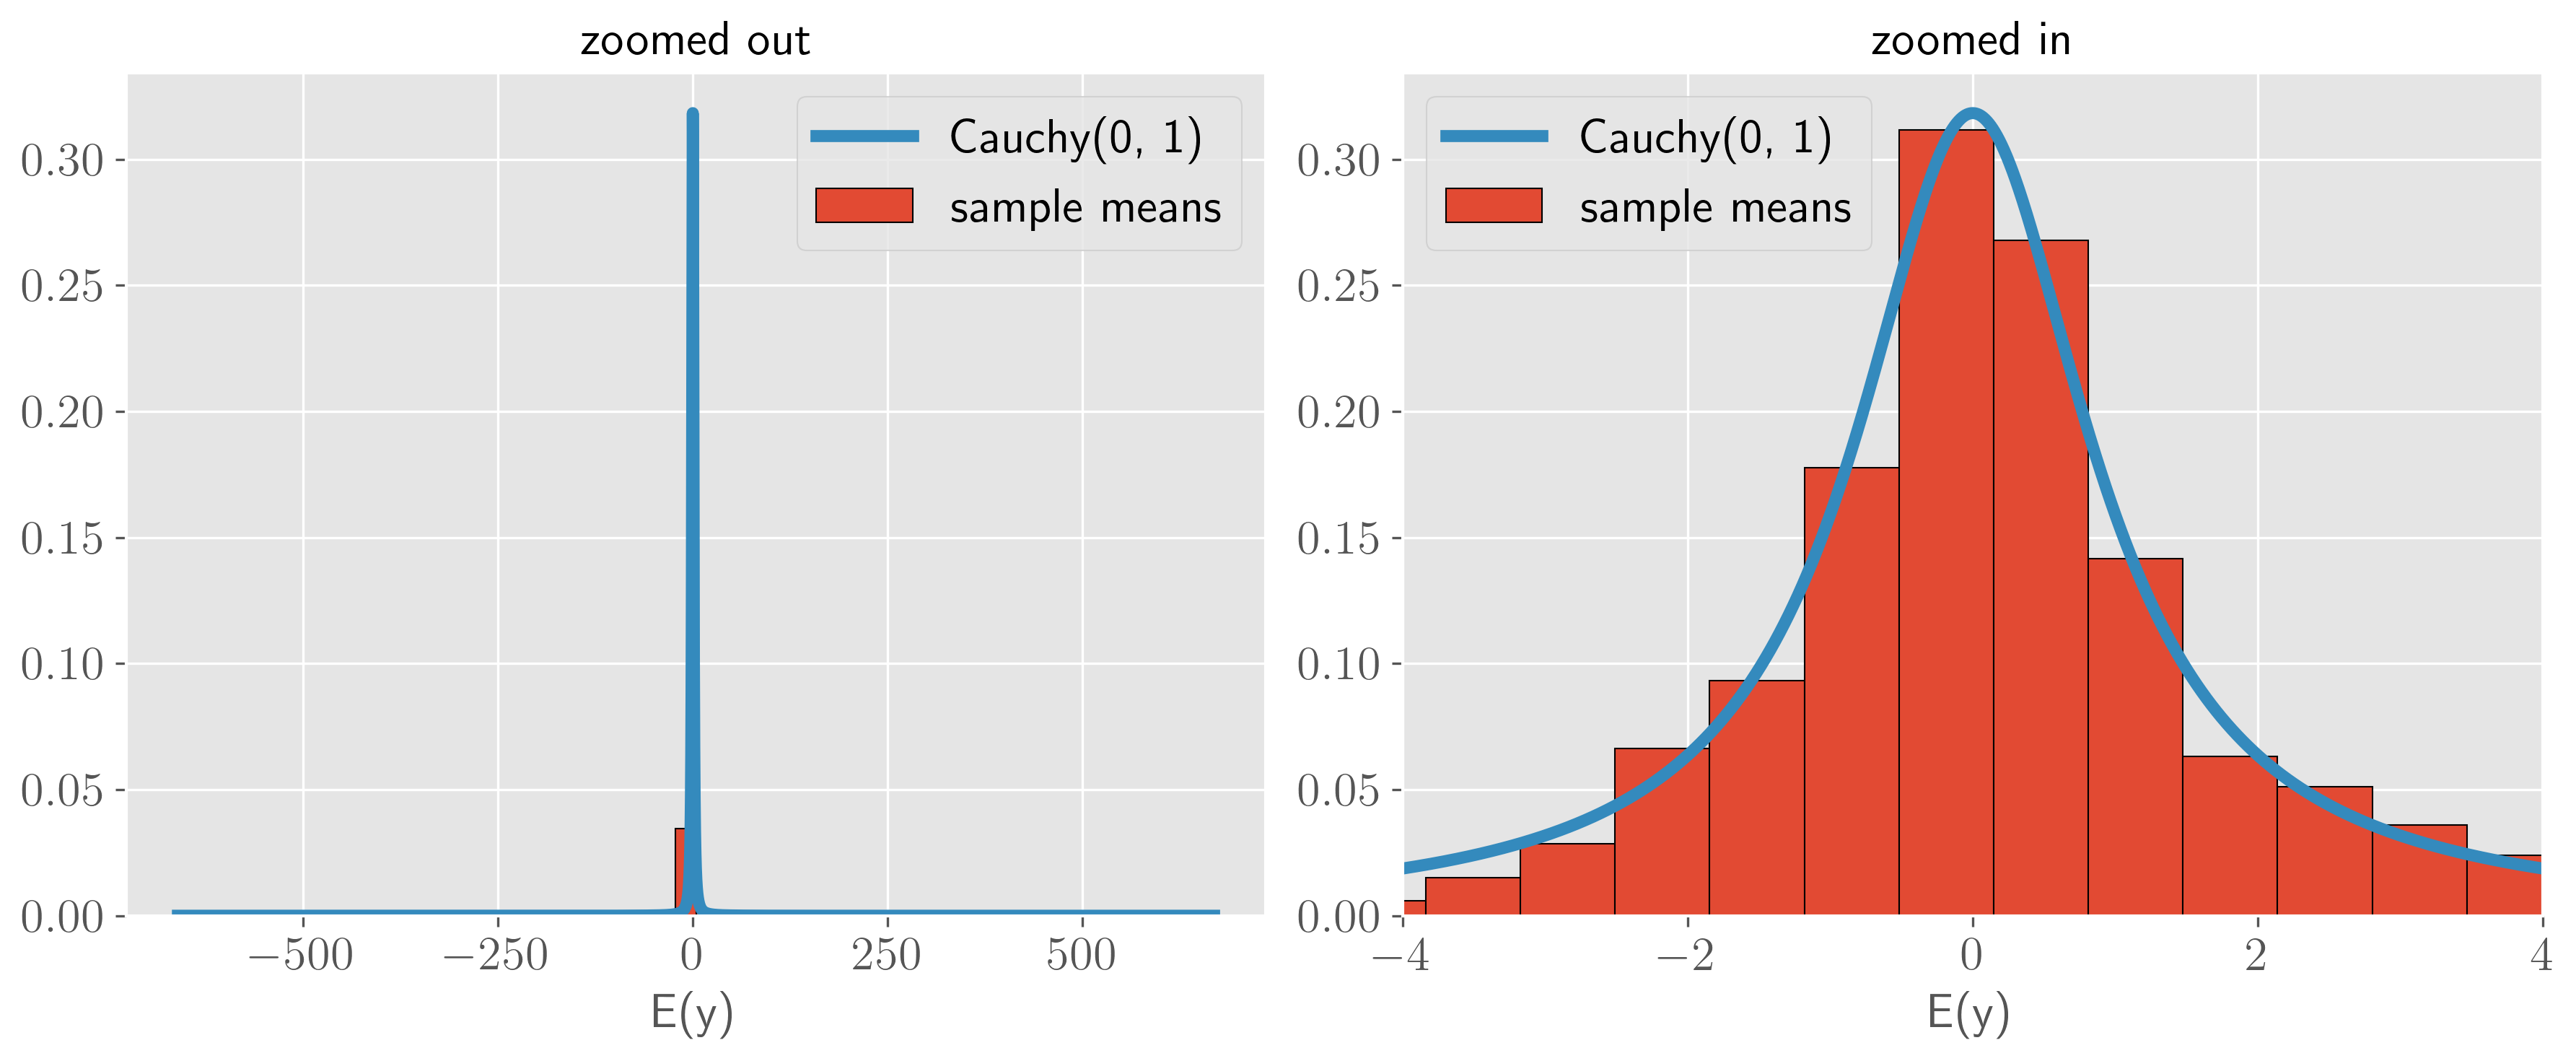
\includegraphics[scale=.55]{homework_2/figures/cauchy_mean.png}
    \caption{Histogram for question (3) (a)}
    \label{fig:my_label}
\end{figure}

\subsection*{Estimate $\theta$ in Cauchy$(\theta, 1)$ using (b) step-wise gradient ascent, (c) Newton-Raphson, and (d) stochastic gradient ascent. }

We need the first and second derivatives of the log likelihood to implement gradient ascent / Newton-Raphson / tochastic gradient ascent. 

\begin{align*} log L(\theta) &= log \prod_{i=1}^n \frac{1}{\pi}\frac{1}{1+(y_i-\theta)^2} \\
&= \sum_{i=1}^n log \frac{1}{\pi}\frac{1}{1+(y_i-\theta)^2} \end{align*}
\begin{align*} \frac{d}{d\theta}log L(\theta) &= \frac{d}{d\theta}\sum_{i=1}^n log \frac{1}{\pi}\frac{1}{1+(y_i-\theta)^2} \\
&=  \sum_{i=1}^n   \frac{2(y_i-\theta)}{1+(y_i-\theta)^2}\end{align*}

\begin{align*} H(\theta) &=\sum_{i=1}^n   \frac{2(y_i-\theta)}{1+(y_i-\theta)^2} \\
&=  \sum_{i=1}^n   \frac{2[(y_i-\theta)^2-1]}{[1+(y_i-\theta)^2]^2} \end{align*}

For gradient ascent and stochastic gradient ascent, we have:

\begin{align*}
    \theta^{(m+1)} = \theta^{(m)} + \gamma \frac{\partial \mathcal{L}(\theta^{(m)})}{\partial \theta}
\end{align*}

For stochastic gradient ascent, we randomly choose a single sample to evaluate the log likelihood at each iteration. For Newton-Raphson:

\begin{align*}
    \theta^{(m+1)} = \theta^{(m)} - H(\theta^{(m)})^{-1} \frac{\partial \mathcal{L}(\theta^{(m)})}{\partial \theta}
\end{align*}

Note that the log likelihood was not strictly concave (its second derivative is not strictly negative). Therefore, the optimizations were repeated several times at different starting values and the run resulting in the highest MLE was chosen. The scripts are attached to this homework.

\end{document}